%!TeX root=20_Hauptteil.tex

%\chapter{Implementierung der Kartierung}
%
%\section{Bildaufnahme}
%
%\subsection{Kamerakalibrierung}
%
%\section{Entzerrung}
%
%\section{Bildverarbeitung}
%
%\section{Kartenerstellung}







\chapter{Implementierung der Kartierung}
\label{cap:kartierung}
In nachfolgenden Kapitel werden die Schritte, welche zur Implementierung der Kartierung notwendig sind, beschrieben.
Hierbei werden Festlegungen getätigt, welche auch direkten Einfluss auf die in Kapitel \ref{cap:lokalisierung} haben. 


\section{Auswahl der Algorithmik}
\section{Auswahl der Algorithmik}
Für die Kartierung werden in dieser Arbeit zwei Ansätze verfolgt.
Zum einen die Live-Kartierung mittels \gls{slam} während des Flugs und zum anderen die Offline-Kartierung durch Aufzeichnung von \gls{ros2}-Bags.
Da die Karte als spätere Referenz für die Lokalisierung des \gls{uav} dient, überträgt sich ihre Genauigkeit unmittelbar auf den Lokalisierungsfehler.
Um eine möglichst genaue Karte zu erhalten und den relativen Fehler der Karte sowie der Lokalisierung gering zu halten, 
kommen ausschließlich optimierungsbasierte \gls{slam}-Methoden zum Einsatz.
Ausschlaggebend für diese Wahl sind die in Kapitel~\ref{sec:slam} beschriebenen Vorteile wie die globale Kartenkorrektur.
Als Nachteil dieser Designentscheidung ist ein erhöhter Rechenaufwand zu nennen.
Dieser macht sich vor allem bei der Live-Kartierung bemerkbar.

In Abbildung \ref{fig:paarweiser_vergleich_slam} werden die in Kapitel \ref{sec:slam_varianten} vorgestellten \gls{slam}-Varianten miteinader verglichen.
Wichtige Entscheidungskriterien sind: 
- Kosten der Hardware
- Gewicht der Hardware
- Vorbereitung 
- Kompatibilität der Versuchsumgebung
- Driftanfälligkeit. 


\begin{table}[htbp]
    \centering
    \footnotesize
    \renewcommand{\arraystretch}{1.3}
    \setlength{\tabcolsep}{4pt}
    \begin{tabular}{l ccccccc c c}
        \toprule
        \textbf{wichtiger als $\rightarrow$}
            & \rotatebox{90}{Kosten Hardware}
            & \rotatebox{90}{Gewicht Hardware}
            & \rotatebox{90}{Vorbereitung}
            & \rotatebox{90}{Kompat. Umgebung}
            & \rotatebox{90}{Driftanfälligkeit}
            & \rotatebox{90}{ROS2-Verfügbarkeit}
            & \rotatebox{90}{Rechenaufwand}
            & \textbf{Summe} & \textbf{\%} \\
        \midrule
        Kosten Hardware        & \cellcolor{black} & 0 & 0 & 0 & 0 & 0 & 1 & 1 & 4{,}8 \\
        Gewicht Hardware       & 1 & \cellcolor{black} & 0 & 0 & 0 & 0 & 1 & 2 & 9{,}5 \\
        Vorbereitung           & 1 & 1 & \cellcolor{black} & 0 & 0 & 1 & 1 & 4 & 19{,}0 \\
        Kompat. Umgebung       & 1 & 1 & 1 & \cellcolor{black} & 1 & 1 & 1 & 6 & 28{,}6 \\
        Driftanfälligkeit      & 1 & 1 & 1 & 0 & \cellcolor{black} & 1 & 1 & 5 & 23{,}8 \\
        ROS2-Verfügbarkeit     & 1 & 1 & 0 & 0 & 0 & \cellcolor{black} & 1 & 3 & 14{,}3 \\
        Rechenaufwand          & 0 & 0 & 0 & 0 & 0 & 0 & \cellcolor{black} & 0 & 0{,}0 \\
        \midrule
        \multicolumn{8}{r}{\textbf{Prüfsumme}} & \textbf{21} & \textbf{100{,}0} \\
        \bottomrule
    \end{tabular}
    \caption{Paarweiser Vergleich zur Gewichtung der Auswahlkriterien.
    Eine~1 bedeutet, dass das Kriterium der Zeile wichtiger ist als das der Spalte.}
    \label{tab:paarweiser_vergleich}
\end{table}
\FloatBarrier


\begin{table}[htbp]
    \centering
    \footnotesize
    \renewcommand{\arraystretch}{1.3}
    \setlength{\tabcolsep}{4pt}
    \begin{tabular}{l ccccccc c c}
        \toprule
        \textbf{wichtiger als $\rightarrow$}
            & \rotatebox{90}{Kosten Hardware}
            & \rotatebox{90}{Gewicht Hardware}
            & \rotatebox{90}{Vorbereitung}
            & \rotatebox{90}{Kompat. Umgebung}
            & \rotatebox{90}{Driftanfälligkeit}
            & \rotatebox{90}{ROS2-Verfügbarkeit}
            & \rotatebox{90}{Rechenaufwand}
            & \textbf{Summe} & \textbf{\%} \\
        \midrule
        Kosten Hardware        & \cellcolor{black} & 0 & 0 & 0 & 0 & 0 & 1 & 1 & 4{,}8 \\
        Gewicht Hardware       & 1 & \cellcolor{black} & 0 & 0 & 0 & 0 & 1 & 2 & 9{,}5 \\
        Vorbereitung           & 1 & 1 & \cellcolor{black} & 0 & 0 & 1 & 1 & 4 & 19{,}0 \\
        Kompat. Umgebung       & 1 & 1 & 1 & \cellcolor{black} & 1 & 1 & 1 & 6 & 28{,}6 \\
        Driftanfälligkeit      & 1 & 1 & 1 & 0 & \cellcolor{black} & 1 & 1 & 5 & 23{,}8 \\
        ROS2-Verfügbarkeit     & 1 & 1 & 0 & 0 & 0 & \cellcolor{black} & 1 & 3 & 14{,}3 \\
        Rechenaufwand          & 0 & 0 & 0 & 0 & 0 & 0 & \cellcolor{black} & 0 & 0{,}0 \\
        \midrule
        \multicolumn{8}{r}{\textbf{Prüfsumme}} & \textbf{21} & \textbf{100{,}0} \\
        \bottomrule
    \end{tabular}
    \caption{Paarweiser Vergleich zur Gewichtung der Auswahlkriterien.
    Eine~1 bedeutet, dass das Kriterium der Zeile wichtiger ist als das der Spalte.}
    \label{tab:paarweiser_vergleich}
\end{table}
\FloatBarrier












\begin{figure}[htbp]
    \centering
    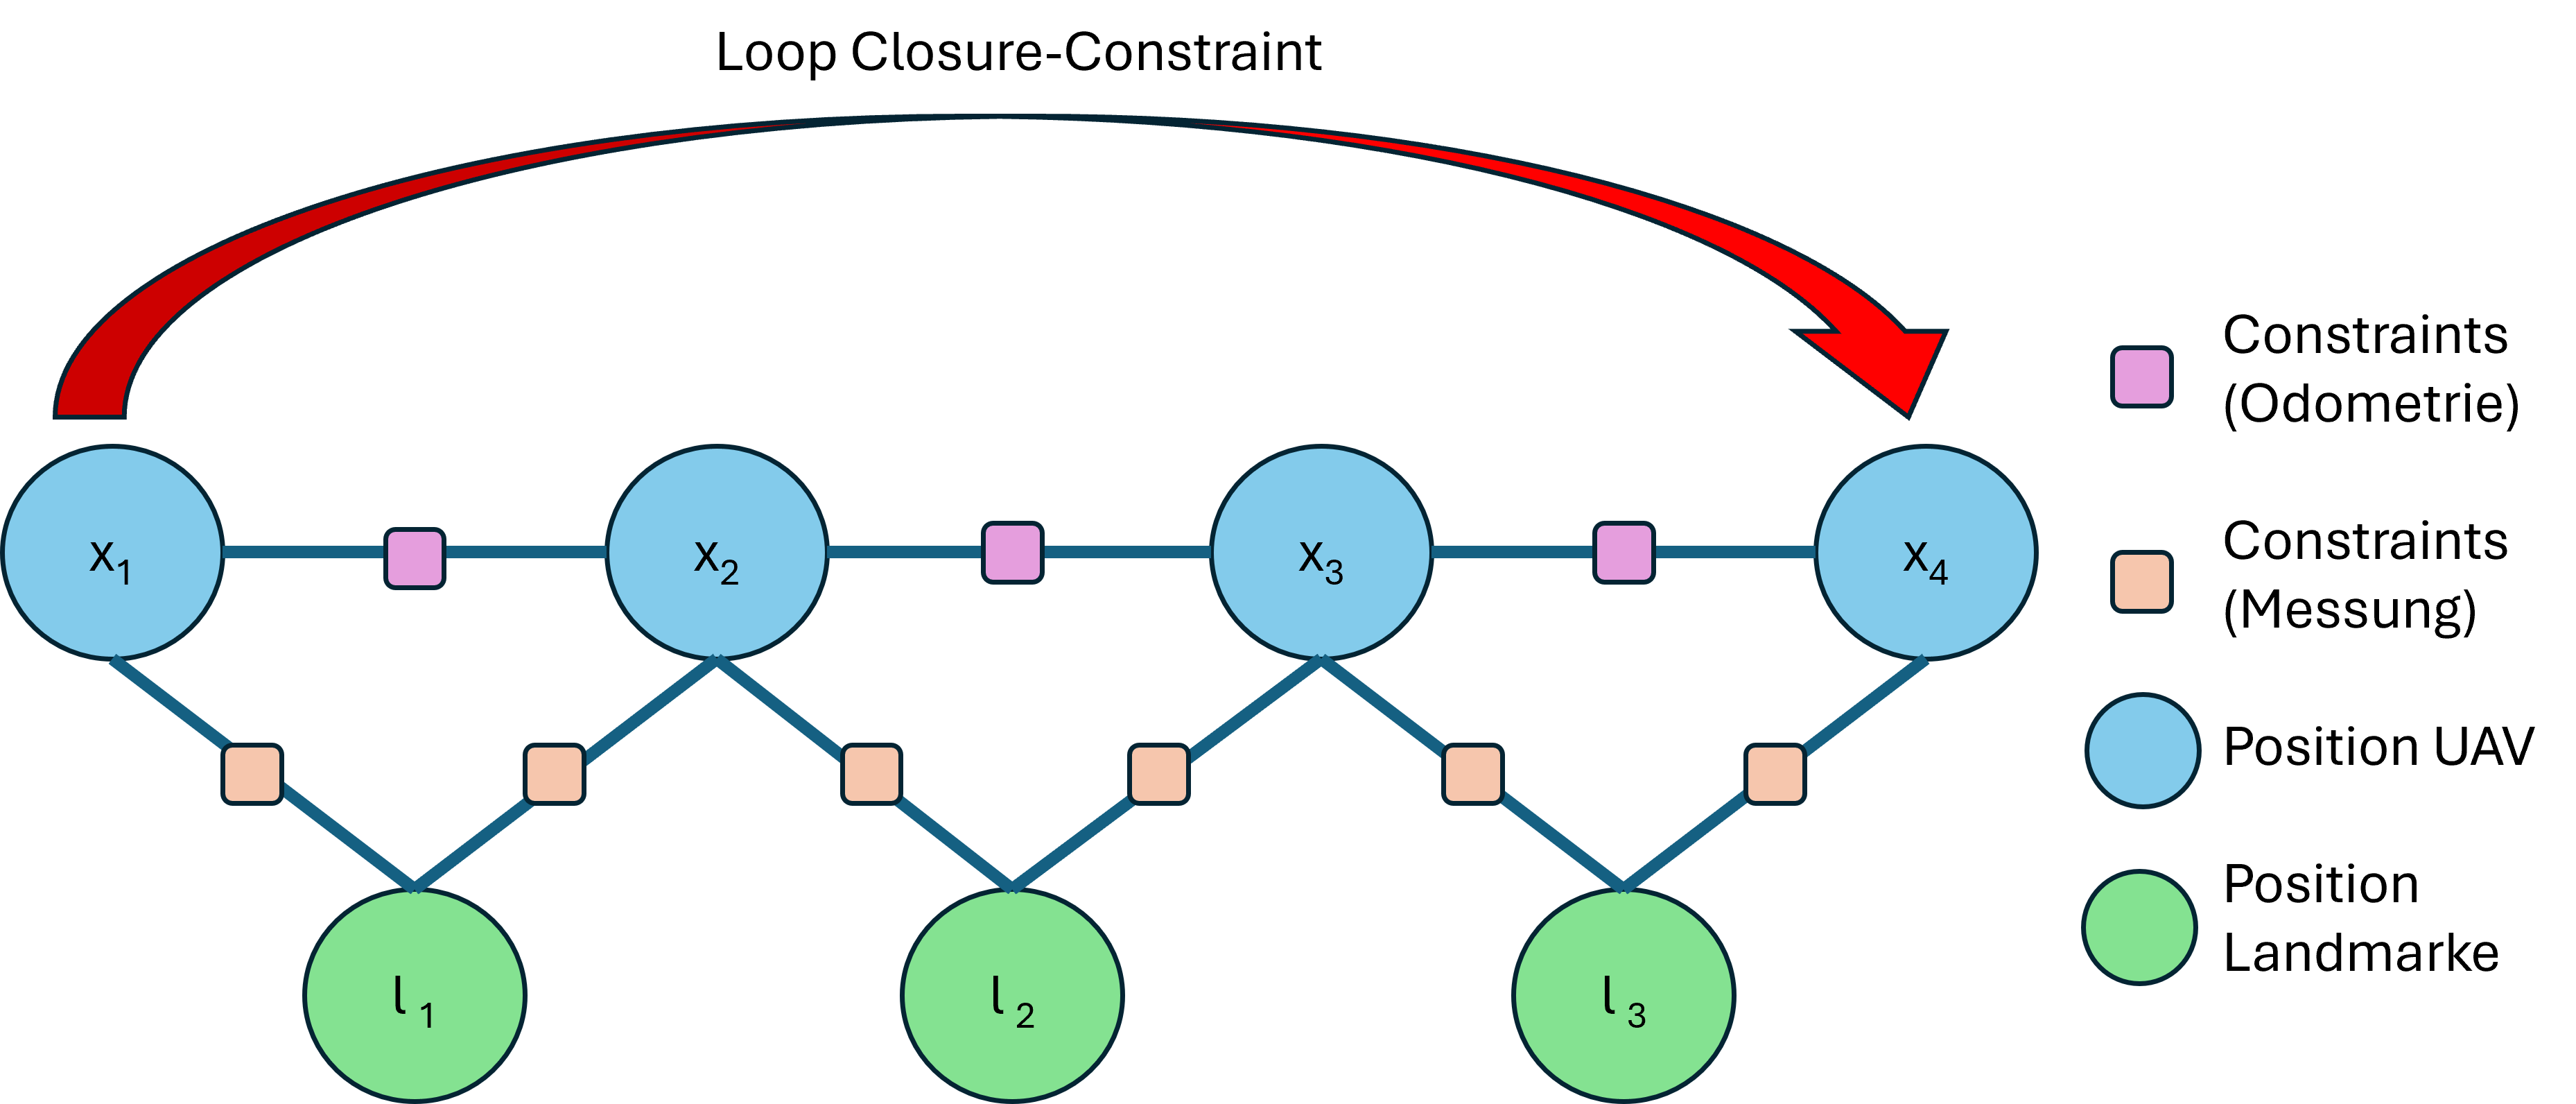
\includegraphics[width=1.0\textwidth]{Bilder/Faktorgraph_vereinfacht.png}
    \caption{Vereinfachter Faktorgraph eines \gls{slam}-Problems, 
    vgl.~\cite{Lai2022}, \cite{Dellaert2017}, \cite{Cai2024}}
    \label{fig:paarweiser_vergleich_slam}
\end{figure}
\FloatBarrier


Für die Kartierung werden in dieser Arbeit zwei Ansätze verfolgt. Zum einen die Live-Kartierung mittels \gls{slam} Algorithmik und zum andern die 
offline Kartierung.
Bei der Live-Kartierung soll es möglich sein, eine Kartierung im Flugbetrieb aufzunehmen.
Die Karte wird nicht im Flug, sondern vorab in einem mehrstufigen Offline-Verfahren erstellt.
Der Ablauf gliedert sich in drei aufeinanderfolgende Stufen, die jeweils als eigenes Launch-File umgesetzt sind und über ROS2-Bags miteinander verbunden werden.
In der ersten Stufe werden die Kamerabilder aufgenommen, entzerrt und in einem Bag aufgezeichnet.
In der zweiten Stufe werden die Marker offline aus den aufgezeichneten Bildern detektiert und gemeinsam mit den Bildern in einem zweiten Bag abgelegt.
In der dritten Stufe werden die Markerlagen aus den Detektionen zu einer konsistenten Karte optimiert.
Die Aufteilung in einen Offline-Ablauf erlaubt es, die Detektion mit reduzierter Abspielgeschwindigkeit auszuführen und den gesamten Vorgang reproduzierbar aus denselben Eingangsdaten zu wiederholen.

% TODO: Abbildung -- Schema des dreistufigen Ablaufs (Bag -> Bag -> Karte).


\begin{table}[htbp]
    \centering
    \renewcommand{\arraystretch}{1.4}
    \begin{tabularx}{\textwidth}{l X X X X}
        \toprule
        \textbf{Verfahren} & \textbf{Kosten} & \textbf{Vorbereitung} & \textbf{Kompatibilität Versuchsumgebung} & \textbf{ROS2-Pakete} \\
        \midrule
        \gls{vo} / \gls{vio}
            & gering, nur Kamera bzw. Kamera mit \gls{imu}
            & keine Umgebungsvorbereitung nötig
            & gering, setzt strukturierte Umgebung voraus, driftbehaftet
            & vorhanden \\
        \addlinespace
        Optimierungs\-basiertes \gls{slam}
            & gering bis mittel, je nach Sensorik
            & keine Umgebungsvorbereitung, hoher Konfigurationsaufwand
            & eingeschränkt, abhängig von Textur und Wiedererkennung
            & vorhanden \\
        \addlinespace
        Fiducial-Marker
            & gering, gedruckte Marker und Kamera
            & einmaliges Anbringen und Einmessen der Marker
            & hoch, unabhängig von Umgebungstextur, absoluter Bezug
            & vorhanden \\
        \bottomrule
    \end{tabularx}
    \caption{Paarweiser Vergleich der betrachteten Lokalisierungsverfahren hinsichtlich der Auswahlkriterien}
    \label{tab:verfahrensvergleich}
\end{table}
\FloatBarrier






\section{Auswahl des Lokalisierungsverfahrens}
\label{sec:auswahl_verfahren}
Für die Innenraumlokalisierung des \gls{uav} kommen grundsätzlich mehrere der in den Grundlagen beschriebenen Verfahren in Frage.
Im Folgenden werden ihre Vor- und Nachteile im Hinblick auf die konkrete Anwendung gegenübergestellt, um die Wahl des eingesetzten Verfahrens zu begründen.

\subsection*{Visuelle Odometrie und visuell-inertiale Odometrie}
Die visuelle Odometrie benötigt keine vorbereitete Umgebung und liefert ohne zusätzliche Infrastruktur eine fortlaufende Bewegungsschätzung.
In der visuell-inertialen Variante wird die Robustheit durch die Inertialdaten weiter erhöht, die den metrischen Maßstab sowie Roll- und Nickwinkel stützen.
Diesen Vorteilen stehen jedoch zwei für die vorliegende Anwendung wesentliche Nachteile gegenüber.
Da beide Verfahren keinen absoluten Positionsbezug besitzen, akkumulieren sie über die Zeit einen Drift und sind damit für eine langfristig stabile Innenraumlokalisierung nur bedingt geeignet.
Zudem setzen sie eine strukturierte, texturreiche Umgebung voraus, die in der Versuchsumgebung nicht zuverlässig gegeben ist.

\subsection*{Simultane Lokalisierung und Kartierung}
\gls{slam}-Verfahren erstellen eine Karte der Umgebung und bestimmen gleichzeitig die eigene Position darin.
Durch Loop Closure und die anschließende globale Optimierung können sie den akkumulierten Drift korrigieren und erreichen so eine höhere Konsistenz als die reine Odometrie.
Allerdings teilen optimierungsbasierte \gls{slam}-Verfahren die Abhängigkeit von einer texturreichen Umgebung und erfordern einen deutlich höheren Rechen- und Implementierungsaufwand.
Der spiegelnde Hallenboden und die strukturarmen Flächen der Versuchsumgebung (siehe Abschnitt~\ref{sec:versuchsumgebung}) erschweren sowohl die Merkmalsextraktion als auch die zuverlässige Wiedererkennung bereits besuchter Orte.

\subsection*{Fiducial-Marker}
Fiducial-Marker stellen künstliche Landmarken mit bekannter Position dar und schaffen damit den absoluten Positionsbezug, der den zuvor genannten Verfahren fehlt.
Da jeder Marker eindeutig identifizierbar ist und seine Lage in der Karte bekannt ist, akkumuliert sich kein Drift, solange Marker sichtbar sind.
Die Erkennung ist robust gegenüber strukturarmen Flächen, da nicht die Umgebungstextur, sondern der Marker selbst das auszuwertende Merkmal bildet.
Als Nachteil ist die Umgebung vorzubereiten, indem die Marker angebracht und eingemessen werden müssen.
Für eine räumlich begrenzte, kontrollierte Versuchsumgebung ist dieser einmalige Aufwand jedoch vertretbar.

\subsection*{Begründung der Verfahrenswahl}
Die Gegenüberstellung zeigt, dass die rein relativen Verfahren an den Bedingungen der Versuchsumgebung scheitern: Sowohl visuelle Odometrie als auch optimierungsbasiertes \gls{slam} setzen eine strukturierte Umgebung voraus und liefern, im Fall der Odometrie, keinen driftfreien absoluten Bezug.
Fiducial-Marker umgehen beide Einschränkungen, da sie einen absoluten Positionsbezug bereitstellen und unabhängig von der Umgebungstextur erkannt werden.
Aus diesen Gründen wird die Lokalisierung in dieser Arbeit auf Basis von Fiducial-Markern umgesetzt.














\section{Bildaufnahme}
\label{sec:kartierung_bildaufnahme}
Die Bildaufnahme erfolgt mit einer Logitech~C922 über das ROS2-Paket gscam.
Die Kamera liefert einen MJPEG-Stream mit einer Auflösung von $1920 \times 1080$ Pixeln bei $15\,\text{fps}$.
Die Dekodierung des MJPEG-Streams erfolgt über eine GStreamer-Pipeline auf der CPU mittels \texttt{jpegdec}.
Da die Aufnahme auf einem Laptop ohne NVIDIA-Hardwaredecoder durchgeführt wird, ist die CPU-Dekodierung hier die geeignete Wahl.
Das aufgenommene Bild wird als Topic \texttt{/camera/image\_raw} mit den zugehörigen Kameraparametern \texttt{/camera/camera\_info} bereitgestellt.

Im Anschluss an die Aufnahme werden die Bilder direkt entzerrt (siehe Abschnitt~\ref{sec:kartierung_entzerrung}).
Der erste Bag zeichnet die für die weitere Verarbeitung benötigten Topics auf:
\begin{itemize}
    \item \texttt{/camera/image\_rect} -- das entzerrte Bild,
    \item \texttt{/camera/camera\_info} -- die zugehörigen Kameraparameter,
    \item \texttt{/tf\_static} -- die statischen Koordinatentransformationen.
\end{itemize}
Dieser Bag bildet den Eingang der zweiten Stufe.

\subsection{Kamerakalibrierung}
\label{sec:kalibrieren_kamera}
Die für die Entzerrung benötigten Parameter werden vorab durch eine intrinsische Kalibrierung bestimmt.
Grundlage ist das Lochkameramodell, das die Abbildung eines Raumpunktes auf die Bildebene beschreibt.
Ein Punkt $\mathbf{X} = [X, Y, Z]^\top$ im Kamerakoordinatensystem wird dabei auf den Bildpunkt $[u, v]^\top$ abgebildet:
\begin{equation}
    s
    \begin{bmatrix} u \\ v \\ 1 \end{bmatrix}
    =
    \mathbf{K}
    \begin{bmatrix} X \\ Y \\ Z \end{bmatrix},
    \qquad
    \mathbf{K} =
    \begin{bmatrix}
        f_x & 0   & c_x \\
        0   & f_y & c_y \\
        0   & 0   & 1
    \end{bmatrix},
    \label{eq:lochkamera}
\end{equation}
mit dem Skalierungsfaktor $s$, den Brennweiten $f_x, f_y$ und dem Bildhauptpunkt $(c_x, c_y)$.
Die Matrix $\mathbf{K}$ wird als Kameramatrix bezeichnet und fasst die intrinsischen Parameter zusammen.

Reale Objektive weichen vom idealen Lochkameramodell ab und erzeugen eine Verzeichnung.
Diese wird über das Modell plumb\_bob beschrieben, das eine radiale und eine tangentiale Komponente umfasst.
Für einen normierten Bildpunkt $(x, y)$ mit $r^2 = x^2 + y^2$ ergibt sich der verzeichnete Punkt $(x_d, y_d)$ zu:
\begin{align}
    x_d &= x\,(1 + k_1 r^2 + k_2 r^4 + k_3 r^6) + 2 p_1 x y + p_2 (r^2 + 2x^2), \\
    y_d &= y\,(1 + k_1 r^2 + k_2 r^4 + k_3 r^6) + p_1 (r^2 + 2y^2) + 2 p_2 x y.
    \label{eq:verzeichnung}
\end{align}
Dabei beschreiben $k_1, k_2, k_3$ die radiale und $p_1, p_2$ die tangentiale Verzeichnung.

Die Kalibrierung bestimmt diese Parameter, indem ein Kalibriermuster bekannter Geometrie aus verschiedenen Blickwinkeln aufgenommen wird.
Über alle erkannten Musterpunkte wird der Reprojektionsfehler minimiert, also die Abweichung zwischen den gemessenen Bildpunkten und den mit den geschätzten Parametern projizierten Punkten.
% TODO: verwendetes Kalibriermuster und Anzahl der Aufnahmen ergaenzen.
Die in dieser Arbeit ermittelten Parameter sind in Tabelle~\ref{tab:kalibrierung} zusammengefasst.

\begin{table}[htbp]
    \centering
    \begin{tabular}{lll}
        \toprule
        \textbf{Parameter} & \textbf{Symbol} & \textbf{Wert} \\
        \midrule
        Brennweite $x$       & $f_x$ & $1436{,}035$ \\
        Brennweite $y$       & $f_y$ & $1435{,}631$ \\
        Hauptpunkt $x$       & $c_x$ & $907{,}441$ \\
        Hauptpunkt $y$       & $c_y$ & $529{,}629$ \\
        Radiale Verzeichnung & $k_1$ & $0{,}020501$ \\
                             & $k_2$ & $-0{,}076950$ \\
                             & $k_3$ & $0{,}0$ \\
        Tangentiale Verz.    & $p_1$ & $-0{,}000463$ \\
                             & $p_2$ & $-0{,}005645$ \\
        \bottomrule
    \end{tabular}
    \caption{Ergebnis der intrinsischen Kamerakalibrierung der Logitech~C922 bei $1920 \times 1080$}
    \label{tab:kalibrierung}
\end{table}
\FloatBarrier

Aus der Kalibrierung wird zusätzlich eine Projektionsmatrix abgeleitet, die die intrinsischen Parameter des entzerrten Bildes beschreibt:
\begin{equation}
    \mathbf{P} =
    \begin{bmatrix}
        1422{,}620 & 0          & 892{,}932 & 0 \\
        0          & 1440{,}023 & 528{,}758 & 0 \\
        0          & 0          & 1         & 0
    \end{bmatrix}.
    \label{eq:projektionsmatrix}
\end{equation}
Diese Matrix wird in den nachfolgenden Schritten anstelle der ursprünglichen Kameramatrix verwendet.

\section{Entzerrung}
\label{sec:kartierung_entzerrung}
Die Entzerrung wird über den Knoten \texttt{rectify\_node} aus dem Paket image\_proc umgesetzt.
Dieser berechnet aus den Kalibrierparametern für jeden Pixel des Ausgabebildes die zugehörige Position im verzeichneten Eingangsbild und entfernt so die durch das Objektiv verursachte Verzeichnung.
Das Ergebnis wird als Topic \texttt{/camera/image\_rect} bereitgestellt.

Nach diesem Schritt ist das Bild bereits entzerrt.
Seine intrinsischen Parameter entsprechen damit der Projektionsmatrix aus Gleichung~\eqref{eq:projektionsmatrix}, und die Verzeichnungskoeffizienten sind null.
Dieser Zusammenhang ist für die nachfolgende Markererkennung entscheidend: Würde dort erneut mit den ursprünglichen Verzeichnungskoeffizienten gerechnet, würde die bereits korrigierte Verzeichnung ein zweites Mal angewendet und die Markerlage systematisch verfälscht.
Aus diesem Grund werden in der Konfiguration der Kartierung als Intrinsics die Werte der Projektionsmatrix eingetragen und die Verzeichnungskoeffizienten auf null gesetzt.

% TODO: Abbildung -- Vergleich Rohbild (verzeichnet) und entzerrtes Bild.

\section{Bildverarbeitung}
\label{sec:kartierung_bildverarbeitung}
Die Markererkennung wird offline auf den aufgezeichneten, entzerrten Bildern ausgeführt.
Dazu wird der Bag der ersten Stufe abgespielt und der Detektionsknoten \texttt{sync\_and\_detect\_node} auf den Bildstrom angewendet.

Das Abspielen erfolgt mit der Option \texttt{-{}-clock} und der Parameter \texttt{use\_sim\_time} ist aktiviert.
Dadurch arbeitet die Detektion mit simulierter Zeit und ist an die Zeitstempel der aufgezeichneten Daten gekoppelt, nicht an die reale Systemzeit.
Die Abspielgeschwindigkeit wird auf den Faktor $0{,}3$ reduziert.
So steht der Detektion pro Bild ausreichend Rechenzeit zur Verfügung, sodass keine Bilder ungenutzt verworfen werden.

Für jeden erkannten Marker werden die Identifikationsnummer sowie die Bildkoordinaten seiner vier Eckpunkte bestimmt und als Topic \texttt{/tagslam/tag\_detections} ausgegeben.
Die Detektionen werden zusammen mit den Bildern, den Kameraparametern, den statischen Transformationen und der simulierten Zeit in einem zweiten, kombinierten Bag aufgezeichnet:
\begin{itemize}
    \item \texttt{/camera/image\_rect},
    \item \texttt{/camera/camera\_info},
    \item \texttt{/tagslam/tag\_detections},
    \item \texttt{/tf\_static},
    \item \texttt{/clock}.
\end{itemize}
Dieser kombinierte Bag enthält alle Eingangsdaten der eigentlichen Kartenerstellung.

\section{Kartenerstellung}
\label{sec:kartierung_tagslam}
Die Kartenerstellung erfolgt mit TagSLAM über den Knoten \texttt{tagslam\_from\_bag}.
Dieser liest den kombinierten Bag ein und schätzt aus den Markerdetektionen die Lage aller Marker zueinander.

\subsection{Optimierungsverfahren}
TagSLAM formuliert das Problem als Faktorgraph und löst es als nichtlineares Ausgleichsproblem.
Gesucht werden die Posen aller Marker sowie die Kamerapose je Bild, die die beobachteten Markerecken bestmöglich erklären.
Für jede beobachtete Markerecke wird der Reprojektionsfehler gebildet, also die Abweichung zwischen der gemessenen Bildkoordinate $\mathbf{z}_{ij}$ und der projizierten Eckposition:
\begin{equation}
    \min_{\{\mathbf{T}_c\}, \{\mathbf{T}_t\}}
    \sum_{i} \sum_{j}
    \left\lVert
        \mathbf{z}_{ij} - \pi\!\left(\mathbf{K}, \mathbf{T}_{c_i}, \mathbf{T}_{t_j}\right)
    \right\rVert^2_{\Sigma},
    \label{eq:tagslam_kost}
\end{equation}
wobei $\mathbf{T}_{c_i}$ die Pose der Kamera im Bild $i$, $\mathbf{T}_{t_j}$ die Pose des Markers $j$ und $\pi(\cdot)$ die Projektion einer Markerecke in die Bildebene bezeichnet.
Die Gewichtung $\Sigma$ ergibt sich aus dem angenommenen Messrauschen, das über den Parameter \texttt{pixel\_noise} mit $1{,}0$ Pixel festgelegt ist.

\subsection{Konfiguration}
Die Konfiguration erfolgt über drei Dateien: die Kameraparameter in \texttt{cameras.yaml}, die Kamerapose in \texttt{camera\_poses.yaml} und die TagSLAM-Konfiguration in \texttt{tagslam\_Lauf2.yaml}.
Die wesentlichen Optimierungsparameter sind in Tabelle~\ref{tab:tagslam_params} zusammengefasst.

\begin{table}[htbp]
    \centering
    \begin{tabular}{ll}
        \toprule
        \textbf{Parameter} & \textbf{Wert} \\
        \midrule
        \texttt{optimizer\_mode}                  & slow \\
        \texttt{pixel\_noise}                      & $1{,}0$ \\
        \texttt{minimum\_viewing\_angle}           & $15{,}0^\circ$ \\
        \texttt{minimum\_tag\_area}                & $2500\,\text{px}^2$ \\
        \texttt{max\_num\_incremental\_opt}        & $10$ \\
        \texttt{max\_subgraph\_error}              & $10{,}0$ \\
        \texttt{subgraph\_abs\_prior\_position\_noise} & $0{,}15$ \\
        \texttt{subgraph\_abs\_prior\_rotation\_noise} & $0{,}15$ \\
        \texttt{use\_approximate\_sync}            & true \\
        \bottomrule
    \end{tabular}
    \caption{Verwendete TagSLAM-Optimierungsparameter}
    \label{tab:tagslam_params}
\end{table}
\FloatBarrier

Der Parameter \texttt{minimum\_viewing\_angle} verwirft Beobachtungen, bei denen der Marker zu schräg zur Kamera steht, da die Eckpunkte dann ungenau bestimmt werden.
Analog schließt \texttt{minimum\_tag\_area} zu kleine und damit zu weit entfernte Marker aus.
Da die Kamera während der Aufnahme bewegt wird und keine externe Odometrie vorliegt, wird sie als nicht-statischer Körper mit einer Pseudo-Odometrie hohen Rauschens (\texttt{fake\_odom}) modelliert, sodass aufeinanderfolgende Kameraposen nicht künstlich gekoppelt werden.

\subsection{Initialisierung der Markerposen}
Die Marker werden mit unterschiedlich starken Vorabinformationen in die Optimierung eingebracht.
Hierbei werden drei Gruppen unterschieden, die sich in Tag-Größe und Stärke des Priors unterscheiden:
\begin{itemize}
    \item \textbf{Tags 0--12} (Größe $0{,}167\,\text{m}$): gut vermessene Startpositionen mit engem Positionsrauschen.
    Tag~0 ist im Ursprung fixiert und definiert das Kartenkoordinatensystem.
    \item \textbf{Tags 13--52} (Größe $0{,}167\,\text{m}$): grobe Startpositionen aus einer Vorabschätzung mit weichem Prior von $0{,}5\,\text{m}$, sodass ihre Lage während der Optimierung angepasst wird.
    \item \textbf{Tags 120--130} (Größe $0{,}232\,\text{m}$): ohne Vorabposition, deren Lage vollständig aus den Beobachtungen bestimmt wird.
\end{itemize}
Bei allen Markern ist die $z$-Koordinate auf null fixiert und die Rotation um die $x$- und $y$-Achse gesperrt, da die Marker eben am Boden liegen.
Lediglich die Position in der Ebene sowie die Rotation um die $z$-Achse bleiben frei.
Diese Einschränkung reduziert die Zahl der freien Parameter und stabilisiert die Optimierung.

\subsection{Ergebnis}
Das Ergebnis ist eine konsistente Karte, die die Lage aller Marker im gemeinsamen Kartenkoordinatensystem beschreibt.
Die optimierte Karte wird in einen Ausgabe-Bag geschrieben und anschließend im Flug für die Lokalisierung verwendet.
% TODO: Abbildung -- optimierte Markerkarte (z. B. RViz-Darstellung der Tags).










